\documentclass{school-22.211-notes}
\date{March  5, 2012}

\begin{document}
\maketitle

\topic{Hemogeneous Resonance Self-Shielding}

\topic{Heterogeneous Geometry Resonant Approximations}
This is probably the most important topic in generating cross section in reactor physics. 

We want to take into account both the spatial and energy structure distributions of flux within each resonance when solving the neutron slowing down problem. 

Model assumptions:
\begin{itemize}
\item All neutron interactions in moderator are purely scattering;
\item Moderator scattering xs is independent of energy;
\item The previous two points together leads to that the slowing down energy source in fuel and moderator is 1/E;
\item Slowing down source is spatially uniform within each region (a fairly accurate assumption);
\item A single resonance absorber species exists only in the fuel;
\item Fuel scattering removes neutrons from resonance energy (that is, narrow resonance model); 
\end{itemize}

\subtopic{Reciprocity Condition}
First we introduce the reciprocity condition. The only assumption we make is that the source is flat. It is independent of geometry. 


where $\tau = \frac{x_1}{\lambda_1} + \frac{x_2}{\lambda_2} = x_1 \Sigma_1 + x_2 \Sigma_2$. 


\subtopic{First Collision Reaction Rate Balance}



\subtopic{Use Reciprocity to Construct 2-Region Balance Equations}


$\sigma_{t,f}(u) = \sigma_{r,f} + \sigma_{pot, f}$, the resonance absorption xs plus the potential scattering xs. 


\subtopic{Heterogeneous/Homogeneous Equivalence}
\hi{Heterogeneous/Homogeneous Equivalence} says that we can compare the heterogeneous energy shape of the flux in the fuel: 


\subtopic{Bell's Refinements of the Wigner's Collision Probability}
Bell Factor: 



\subtopic{Arrays of Rods, Dancoff Factor}
Notice our model so far is an isolated pin (that is, a fuel pin surrounded by an almost infinite moderator). Now we are going to discuss arrays of rods. We define the \hi{Dancoff Factor C}:
\eqn{ C = 1 - \frac{ \left. P_{f\to f} \right|_{\mbox{isolated rods}}}{ \left. P_{f\to f} \right|_{\mbox{arrays of rods}}}   }
LWRs typically have a C of 0.3. Know how to get C from the plot. 


C changes the coefficient in front of the escape xs $\sigma_e \to \frac{(1-C)b}{1-C + Cb} \sigma_e$. For a typical PWR pin, that is reduce $\sigma_e$ to 0.745 of it. \ce{^{235}U}'s xs is 65 barns [FIXME].

\subtopic{Carlvik's Refinements of the Bell's Collision Probability}
Carlvik's two-term approximation is what is actually used in production tools nowaday. To use it, we essentially look up the resonance integral (or group xs) twice, once with $\sigma_e$ multiplied by $\alpha_1$ and the second time with $\sigma_e$ multiplied by $\alpha_2$, each of them are simple functions of the Dancoff factor. To double check, we let Dancoff factor to go to 1, and there should be no escape from the fuel; let Dancoff factor go to 0, we should get isolated rod. 




\topic{HW4: Real Application of Resonance Model}



\lecture{Exam 1 Review}
Know how to interprete thermal scattering pdf and cdf. 

Questions would be based on understanding of the physics. 

Part 1: Background Info (see Ch 1-3 from Reuss)
\begin{enumerate}
\item Number Density
\item Flux
\item Lethargy
\item Mean free path
\item 1/v, 1/E.
\item Maxwellian shapes.
\end{enumerate}


Part 2: Monte Carlo code:
\begin{enumerate}
\item Asymptotic elastic scattering
\item Maxwellian thermal elastic scattering
\item Simple bound thermal scattering
\item SLBW resonance models
\item Doppler broadening
\item Monte Carlo tallies
\item Resonance integrals vs. group cross sections
\item Background (dilution) cross section
\item etc. 
\end{enumerate}


%%%%%%%%%%%%%%%%%%%%%%%%% Qualify Exam Start %%%%%%%%%%%%%%%%%%%%%%%%%%%%
\lecture{Facts For Qualify Exam}
\begin{enumerate}
\item Flux = $\frac{n}{\cm^2 \s}.$

\item Fast flux in hydrogen is around $10^{14}$ n/cm$^2$s, and on the order of $10^{12}$n/cm$^2$s for thermal flux. 

\item U235 fission xs at 0.1 eV is about 200 barns; Pu239 fission xs is about 500 barns. In thermal reactors, Pu absorption should be about twice that of uranium. 

\item Capture cross-section as in Figure~\ref{capture-xs}: 
\begin{figure}
  \centering
  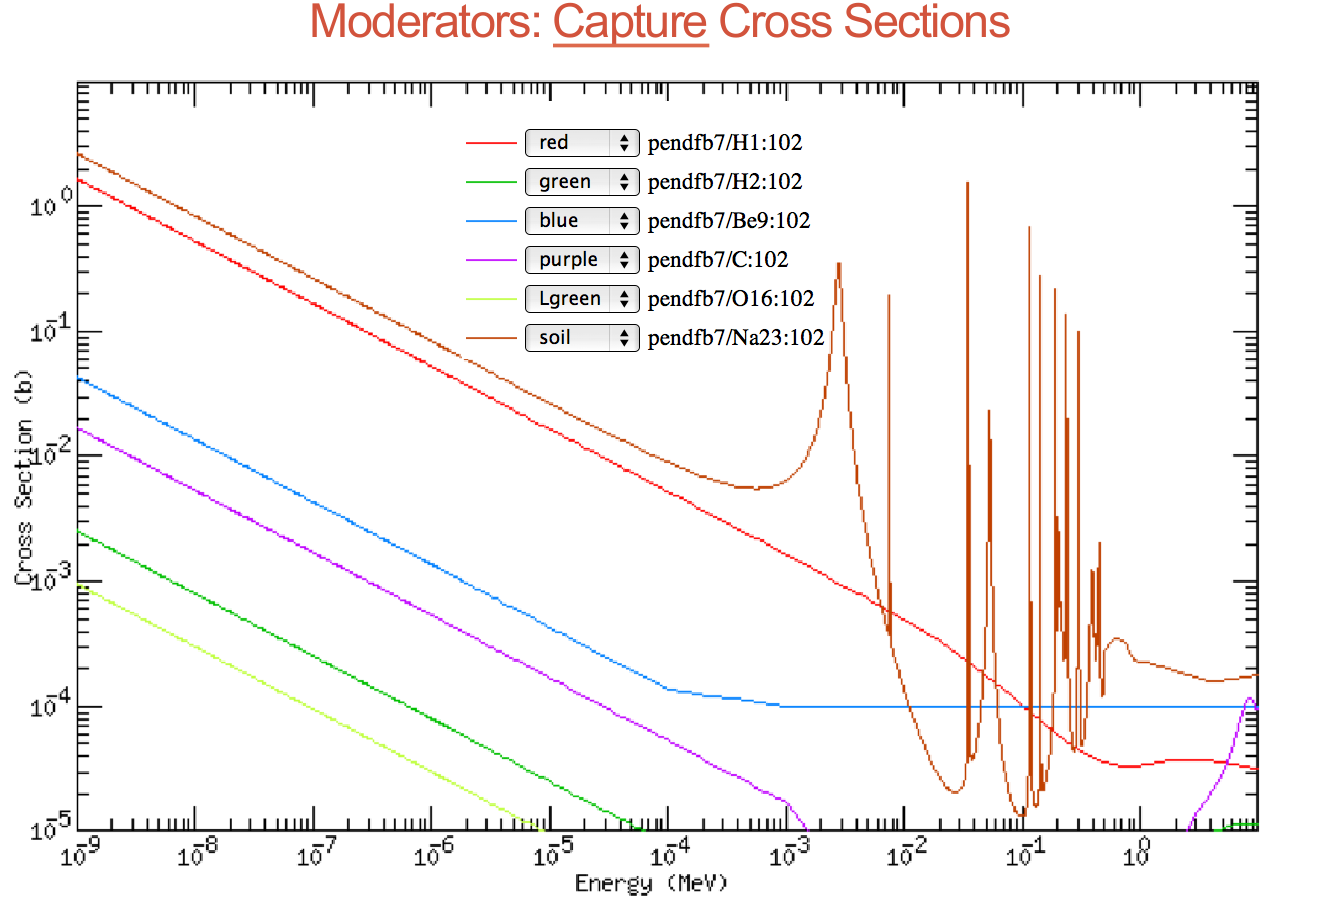
\includegraphics[width=4in]{images/capture-xs.png}
  \\
  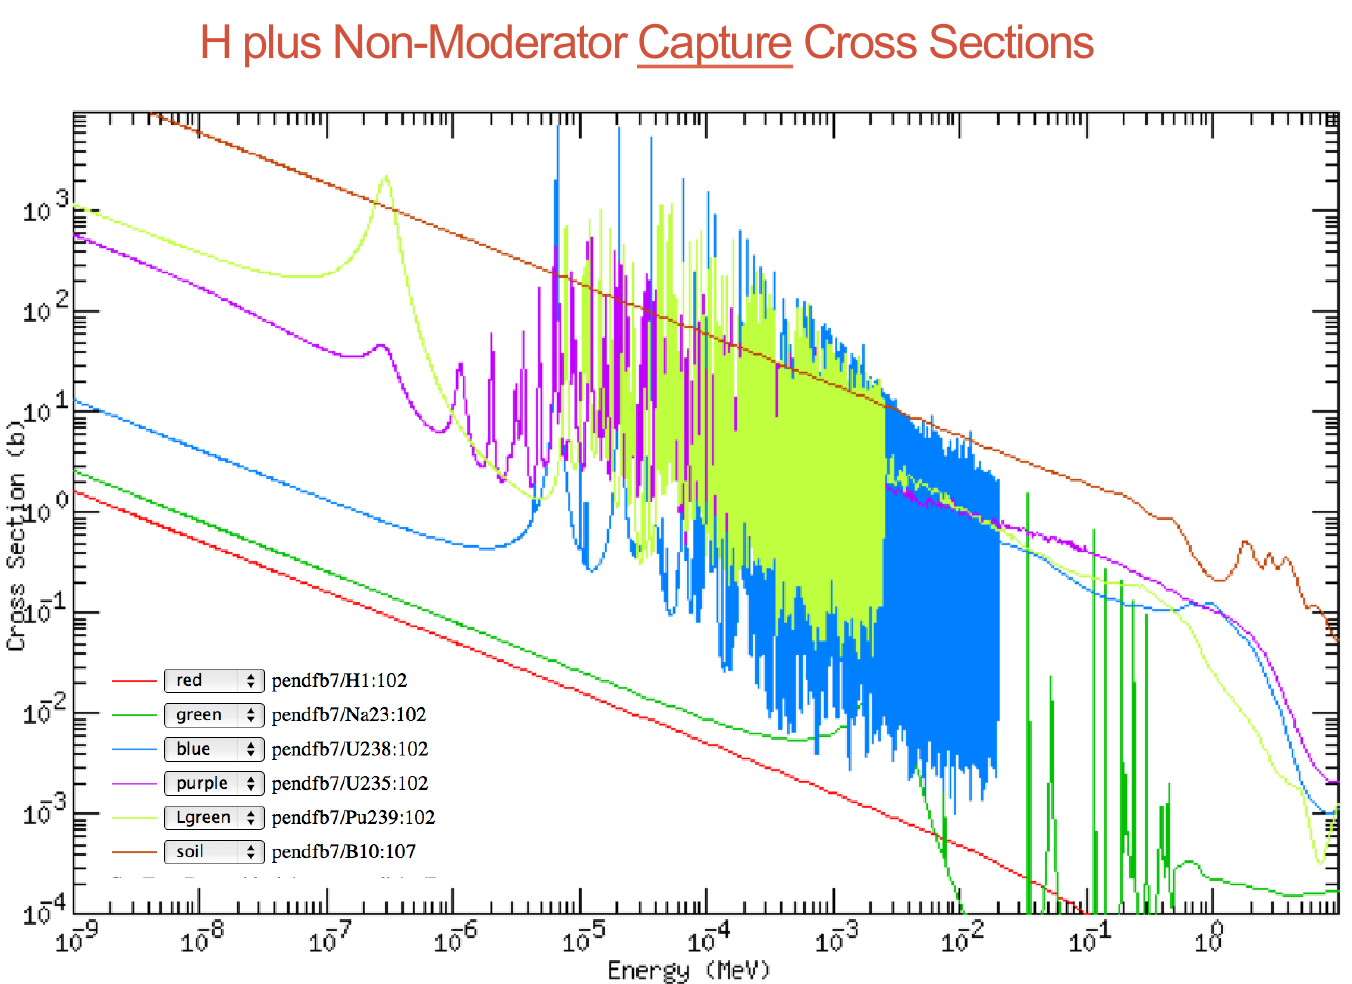
\includegraphics[width=4in]{images/capture-xs-2.png}
  \caption{Capture Cross Section} \label{capture-xs}
\end{figure}
\begin{enumerate}
\item H has no resonance; it has the highest scattering xs in LWR, so we can ignore any other isotopic's neutron scattering.   
\item Na has a huge resonance in 23 keV, and more resonances at higher energies because it is a heavy isotope.
\item Near zero energy,
\eqn{ \sigma(E\to 0) = }
\item Resonance at 6 to 7 eV: U238. 
\item U235's thermal elastic xs is larger than 238's, and they both have resonance around the same range.   
\item A small resonance at .3 eV: Pu239 (its signiture is a super low energy scattering xs). 
\end{enumerate}

\item Given an unknown material type, all we care is to count the nucleus density of each material and look at it's xs. 
\item Average fission neutron energy: 2 MeV; average peak fission energy: 1 MeV; see fission sepctrum. 

\item Core decay heat after 1 day is about 1\% rated. 


\end{enumerate}
%%%%%%%%%%%%%%%%%%%%%%%%% Qualify Exam End %%%%%%%%%%%%%%%%%%%%%%%%%%%%


\end{document}
